\documentclass{article}
\usepackage[utf8]{inputenc}
\usepackage{amsmath,amsthm,amssymb,graphicx,mathtools,tikz,hyperref,enumerate, float, booktabs}

\title{CAI Classification Problem\\Report 4: Implementation III}
\author{Nil Crespo-Peiró, Paco Rahn, Amin Ranem}
\date{2. February 2021}

\begin{document}

\maketitle

\section{Introduction}
After creating the implementation of the initial GUI and the finished Code Base from last report, the following report deals with the final modification of the GUI and the model structures that will be trained in the coming weeks.


\section{Implementation 3}
In this section, the used model structures will be described. Since the Code Base is already implemented, the training of these models and hypertuning has already started in this week. Two different model structures will be used in this regard:
\begin{itemize}
    \item AlexNet: Transfer learning to rebuild the so called ToolNet (part of EndoNet) from the \href{https://arxiv.org/pdf/1602.03012.pdf}{corresponding paper}.
    \item ResNet: Transfer learning using the ResNet-50 model
\end{itemize}

\subsection{AlexNet/ToolNet (part of EndoNet)}
As it has already been mentioned previously, this method will be used as a baseline since it was the one used by the authors of the paper \href{https://arxiv.org/pdf/1602.03012.pdf}{Twinanda et al. 2016}.

\noindent The architecture in this model can be seen in the paper but it is essentially an AlexNet model where the last layer is modified.

\paragraph{\textbf{Results:}}
\noindent Due to certain limitations on the Kaggle Kernels, which has been the platform where the code has been executed, only 37 videos could be trained initially. The initial results were far from optimal since we achieved a training accuracy of a little over 20\% and a test accuracy of approximately 7\%.\\
\noindent In spite of that, the hyperparameter tuning phase began. The goal in this phase is to tune the parameters in order to obtain a high training accuracy in a dataset with very few data (5 videos), and therefore overfit the model. This way the results would not take too much time to get calculated and one could see if these selected parameters were working towards the goal of obtaining a high training accuracy or not.\\
\noindent Once we got really good training accuracy results, the goal was to increase the dataset and check if the model had still good results. A dataset of 20 videos was first used and the model obtaining a 96.76\% training accuracy and still a good 61\% test accuracy. 
\noindent After that, a larger dataset was used (37 videos, the maximum right now that Kaggle was able to load) and got slightly worse results: 89.3\% training accuracy and approximately the same test accuracy. \\
\noindent Looking at this results was obvious that the parameter choices were not the optimal ones so more hyperparameter tuning has to be made for the next report.

\begin{table}[H]
\resizebox{\columnwidth}{!}{%
\begin{tabular}{@{}lllllllllll@{}}
\toprule
\textbf{Model \#} & \textbf{\# videos} & \textbf{\# epochs} & \textbf{learning\_rate} & \textbf{batch\_size} & \textbf{weight\_decay}    & \textbf{train\_acc} & \textbf{train\_loss} & \textbf{val\_acc} & \textbf{val\_loss} & \textbf{test\_acc}    \\ \midrule
\textbf{1}        & 37                 & 30                 & 1e-3                    & 100                  & \multicolumn{1}{l|}{0.75} & 29.33\%             & 0.003332             & 31.23\%           & 0.003474           & \multicolumn{1}{c}{-} \\
\textbf{2}        & 5                  & 300                & 5e-3                    & 200                  & \multicolumn{1}{l|}{0.5}  & 21.45\%             & 0.006631             & 6.85\%            & 0.006808           & \multicolumn{1}{c}{-} \\
\textbf{3}        & 5                  & 60                 & 1e-2                    & 50                   & \multicolumn{1}{l|}{0.5}  & 30.19\%             & 0.01309              & 26.94\%           & 0.01347            & \multicolumn{1}{c}{-} \\
\textbf{4}        & 5                  & 30                 & 1e-3                    & 50                   & \multicolumn{1}{l|}{0.9}  & 17.81\%             & 0.007252             & 6.486\%           & 0.007888           & \multicolumn{1}{c}{-} \\
\textbf{5}        & 5                  & 60                 & 1e-4                    & 32                   & \multicolumn{1}{l|}{1e-3} & 98.89\%             & 0.0002176            & 37.05\%           & 0.01546            & 47\%                  \\
\textbf{6}        & 20                 & 60                 & 1e-4                    & 32                   & \multicolumn{1}{l|}{1e-3} & 96.76\%             & 0.0004687            & 56.84\%           & 0.01028            & 61\%                  \\
\textbf{7}        & 37                 & 10                 & 1e-4                    & 32                   & \multicolumn{1}{l|}{1e-3}                      & 89.30\%             & 0.001431             & 72.99\%           & 0.004042           & 61\%                  \\ \bottomrule
\end{tabular}%
}
\caption{All the specifications for all models used in the hyperparameter tuning phase can be observed}
\end{table}

\subsection{ResNet}
The idea to test transfer learning using ResNet-50 is based on the Cholecystectomy Cataract lecture from the Deep Learning for Medical Imaging (DLMI) course where the ZIB-Net was introduced. The ZIB-Net used two different network architectures (AlexNet and ResNet). The results of the ZIB-Net showed that the ResNet-50 based model could achieve a higher accuracy then the AlexNet.\\
In a first implementation the ResNet-18 was used. Transfer Learning was done by replacing the FC-Layers and fine-tune all parameters of the network. By switching to the ResNet-50 the accuracy was slightly improved. Still with the initial hyperparameters, that can be seen in table \ref{table:resnetres}, the performance was not good and the model was not capable of fitting the training data.\\
Therefore the same approach as for the AlexNet was chosen, with the same focus on weight-decay and learning-rate. In contrast to the AlexNet, the ResNet was not able to fit the training data that fast. The best results are summarized in table \ref{table:resnetres}. The biggest effect was achieved by decreasing the weight-decay. Better results may could be achieved with longer epochs or bigger training data sets.\\
Due to the limited GPU availability, the hyperparameter optimizations had to be stopped at that point. For the rest of the project the focus will mainly lie on the optimization of the AlexNet.

\begin{table}[H]
\label{table:resnetres}
\resizebox{\columnwidth}{!}{%
\begin{tabular}{@{}lllllllllll@{}}
\toprule
\textbf{Model \#} & \textbf{\# videos} & \textbf{\# epochs} & \textbf{learning\_rate} & \textbf{batch\_size} & \textbf{weight\_decay}    & \textbf{train\_acc}  & \textbf{val\_acc} & \textbf{test\_acc}    \\ \midrule
\textbf{1}        & 37                 & 30                 & 1e-4                    & 100                  & \multicolumn{1}{l|}{0.75} & 30.16\%                      & 38.63\%                           & 29\%   \multicolumn{1}{c}{-} \\
\textbf{2}        & 5                  & 15                & 1e-4                    & 30                  & \multicolumn{1}{l|}{0.01}  & 58.61\%                       & 28.6\%                            & 30\%       \multicolumn{1}{c}{-} \\
\textbf{3}        & 5                  & 15                 & 1e-4                    & 30                   & \multicolumn{1}{l|}{5e-3}  & 60.2\%                     & 40.2\%                            & 43\%      \multicolumn{1}{c}{-} \\
\textbf{4}        & 5                  & 10                 & 1e-3                    & 30                   & \multicolumn{1}{l|}{0.00025}  & 67.22\%                  & 35.07\%                           &   40\%       \multicolumn{1}{c}{-} \\
\textbf{5}        & 5                  & 10                 & 1e-3                    & 30                   & \multicolumn{1}{l|}{5e-5} & 70.2\%                   & 45.24\%                           & 53\%                  \\
\textbf{6}        & 5                 & 10                 & 5e-4                    & 30                   & \multicolumn{1}{l|}{0.000125} & 72.2\%                   & 41.62\%                           & 47\%                  \\
\textbf{7}        & 5                 & 10                 & 5e-3                    & 30                   & \multicolumn{1}{l|}{0}        & 68.7\%                   & 51.2\%                           & 27\%                  \\ \bottomrule
\end{tabular}%
}
\caption{Results for the ResNet-50}
\end{table}

\subsection{First training models}
In this section, the first results regarding the initial training phase of the previously described models will be discussed.

\subsection{Improved User Interface}
Since the first prototype of the GUI, presented in the last report, needed to be modified, this section shows the result of the final GUI that is already linked to the Code Base and can be used for predictions with the corresponding models from above, once they have been trained. One of the major modifications of the GUI are the back steps, were the user can go back to previous windows to change the specifications based on his/her desire. Further, the different information regarding the model and the output are for now just exemplary. This will be replaced automatically, once the models are trained. So predictions are done now with the GUI, however with an exemplary ResNet model trained on 5 videos for 2 epochs.

\subsubsection{First Window: Welcome and start window}
Once the user starts the GUI (for prediction) with the following command 
\texttt{python3 SurgeryToolRecognition.py --use\_gui}, the following Welcome window will be displayed, to welcome the user to the Surgical Tool Recognition System:
\begin{figure}[H]
    \centering
    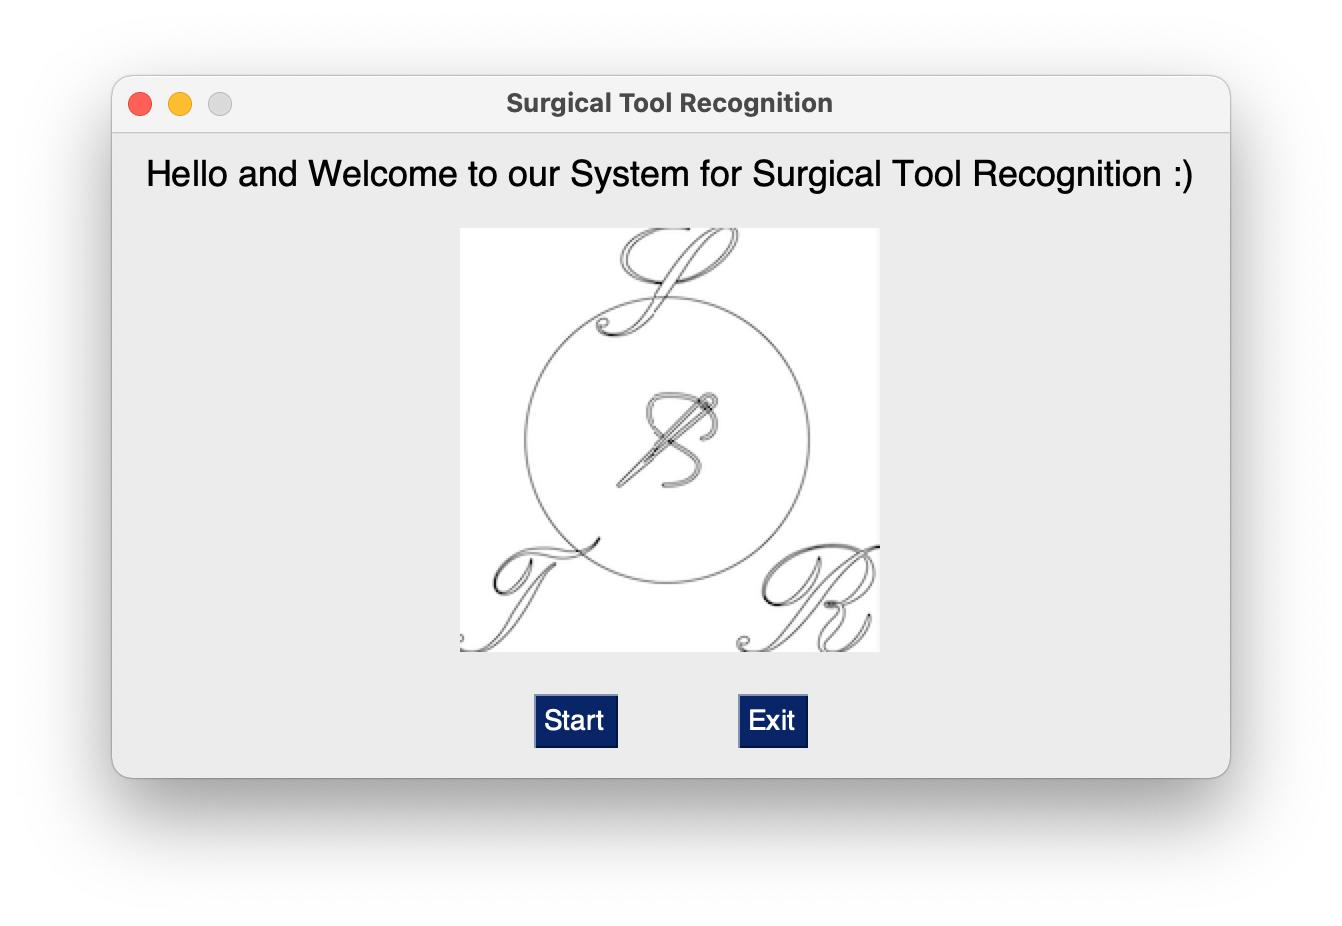
\includegraphics[width = \linewidth]{Welcome_window.jpg}
    \caption{Welcome window}
\end{figure}
\noindent
Once the user hits \texttt{Start}, a new window will be displayed, were the user needs to specify the video he/she wants to load and use the prediction tool for:

\begin{figure}[H]
    \centering
    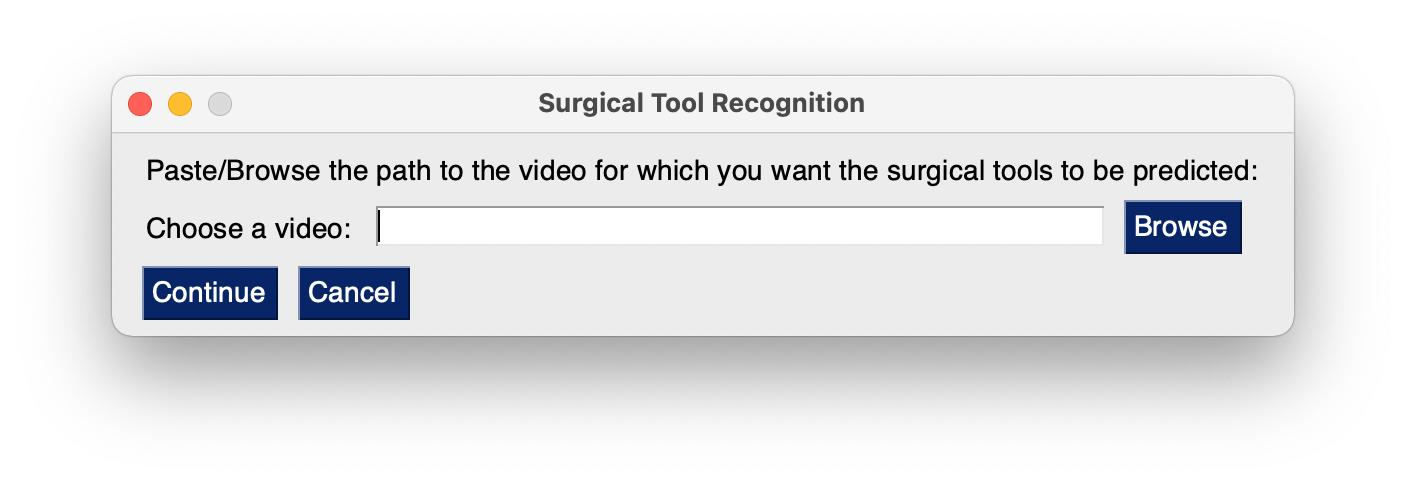
\includegraphics[width = \linewidth]{Browse_window.jpg}
    \caption{Browse window to select the video the user wants the used tools to be predicted in}
\end{figure}
\noindent
Finally, in a popup window, the input file path will be displayed as a small confirmation for the user. Note, that for each following window, the user can go back and perform changes in the previous windows:

\begin{figure}[H]
    \centering
    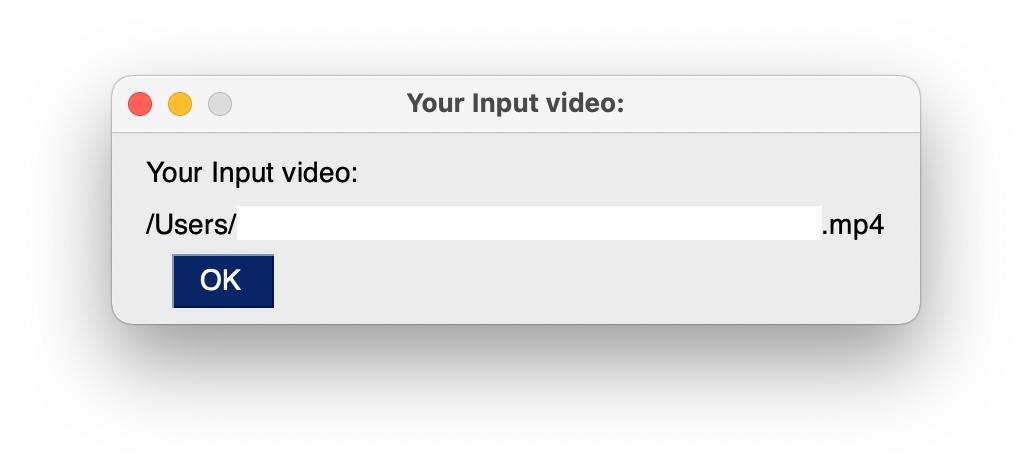
\includegraphics[width = \linewidth]{Confirm_window.jpg}
    \caption{Confirmation popup window}
\end{figure}
\noindent


\subsubsection{Second Window - Video information}
In a next window, information regarding the loaded video will be displayed. If the video has already the desired format, i.e. 1 fps and a frame size of \texttt{(224, 224, 3)}, the user only needs to specify the target path and no transformation will be needed. If the video has not the right format, it will be transformed after the user hits \texttt{Continue}. In such a case, the window displays a corresponding message (Fig: \ref{fig:output}).
\begin{figure}[H]
    \centering
    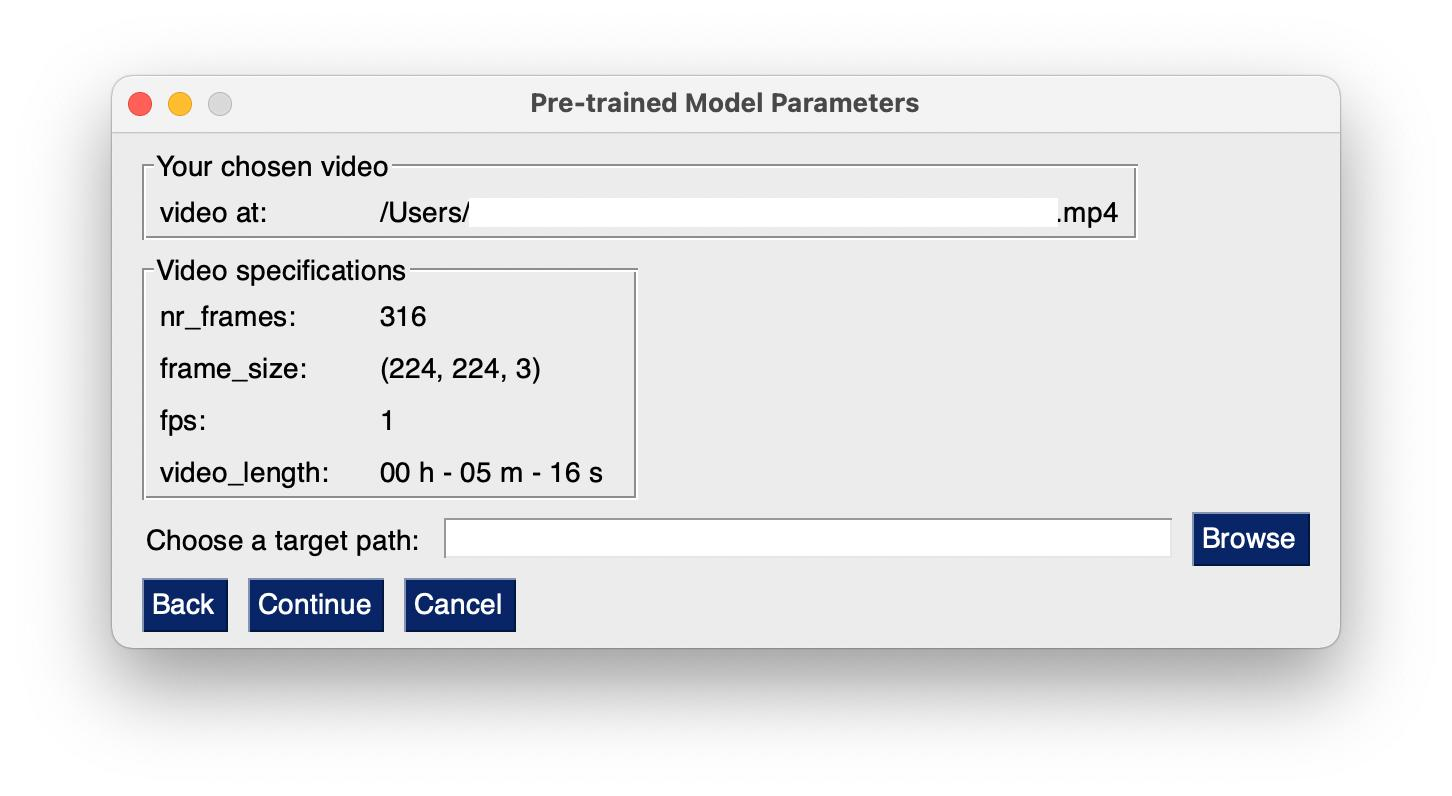
\includegraphics[width = \linewidth]{Output_window.jpg}
    \caption{Video information video -- no transformation needed}
\end{figure}

\begin{figure}[H]
    \centering
    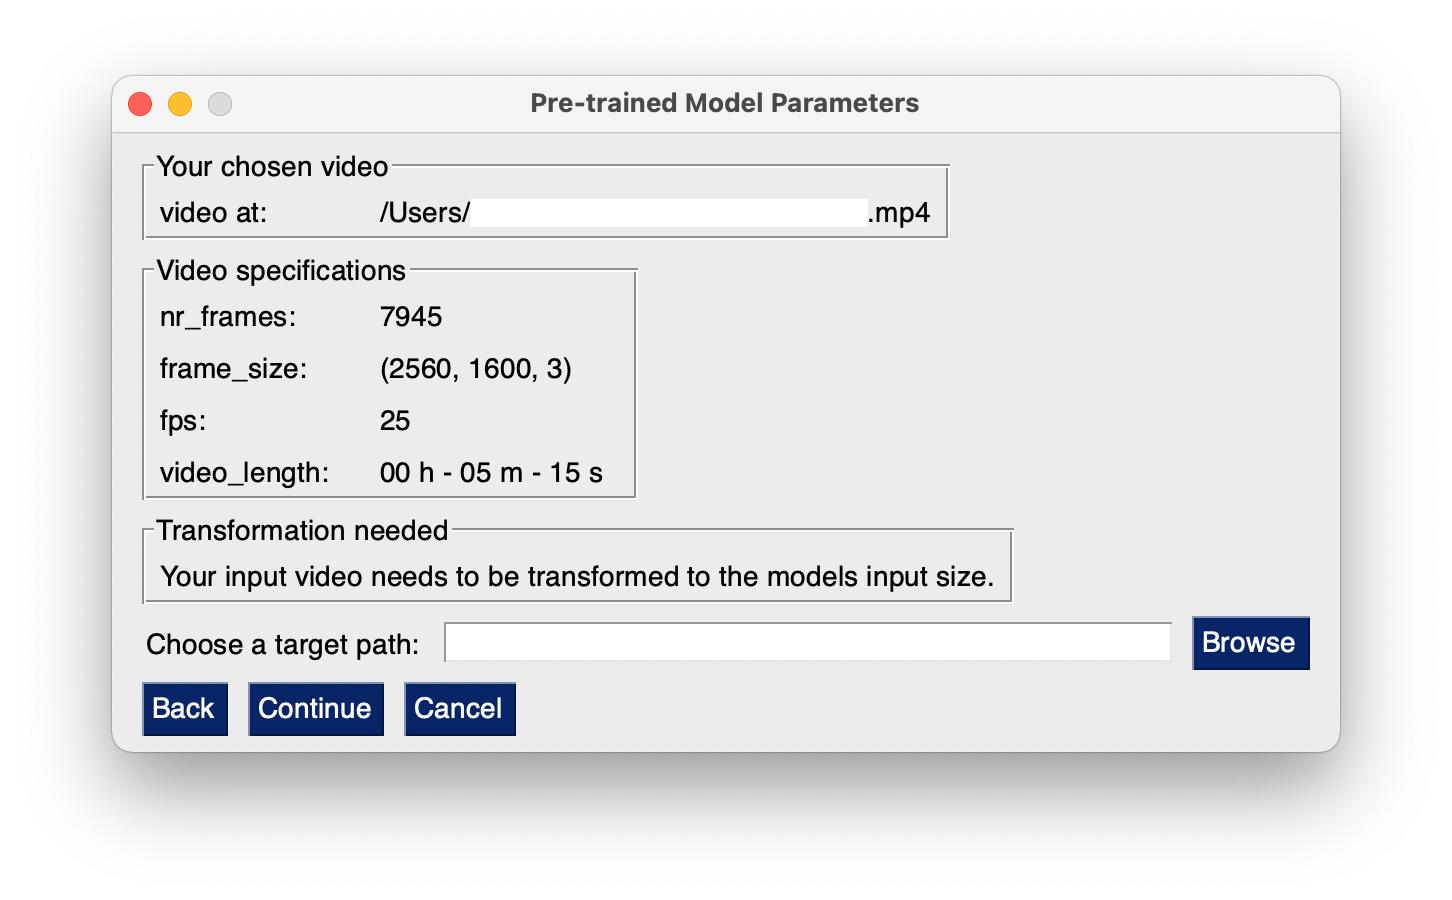
\includegraphics[width = \linewidth]{Transformation_window.jpg}
    \caption{Video information video -- transformation needed}
    \label{fig:output}
\end{figure}

\subsubsection{Third Window - Choose model and device}
In the following window, the user can choose his/her desired model using the Dropdown list and of course the device he/she wants to predict on. If the user chooses a GPU, he/she also has to define the ID which ranges from 0 to 7:

\begin{figure}[H]
    \centering
    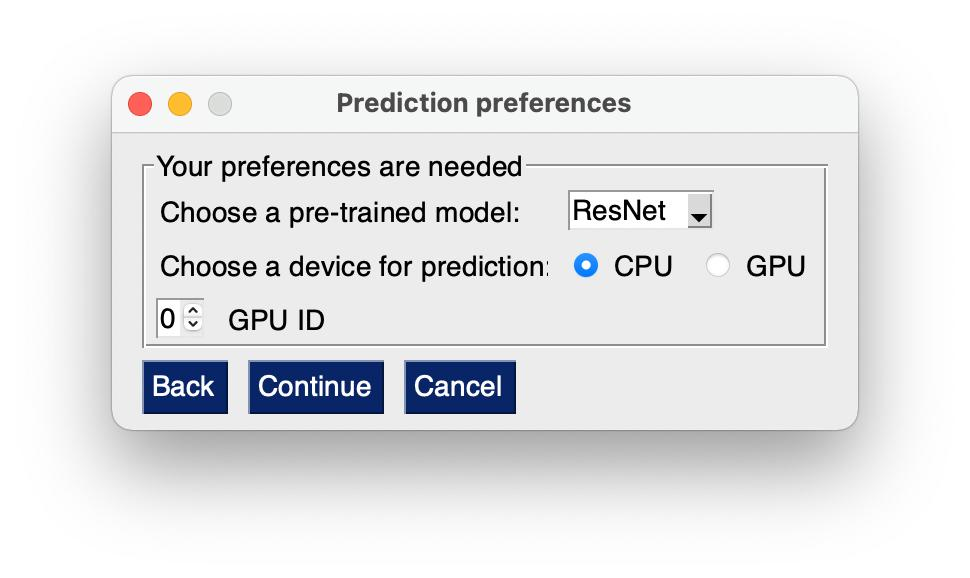
\includegraphics[width = 0.7\linewidth]{Prediction_Preferences.jpg}
    \caption{Window where the user can choose the prediction preferences}
\end{figure}
\noindent
After the chosen model, the parameters and specifications the selected model has been trained on will be displayed. The test accuracy of the model on a previously not seen Dataset will also be displayed. Information in the following window are all exemplary and will be updated once the models have been trained!

\begin{figure}[H]
    \centering
    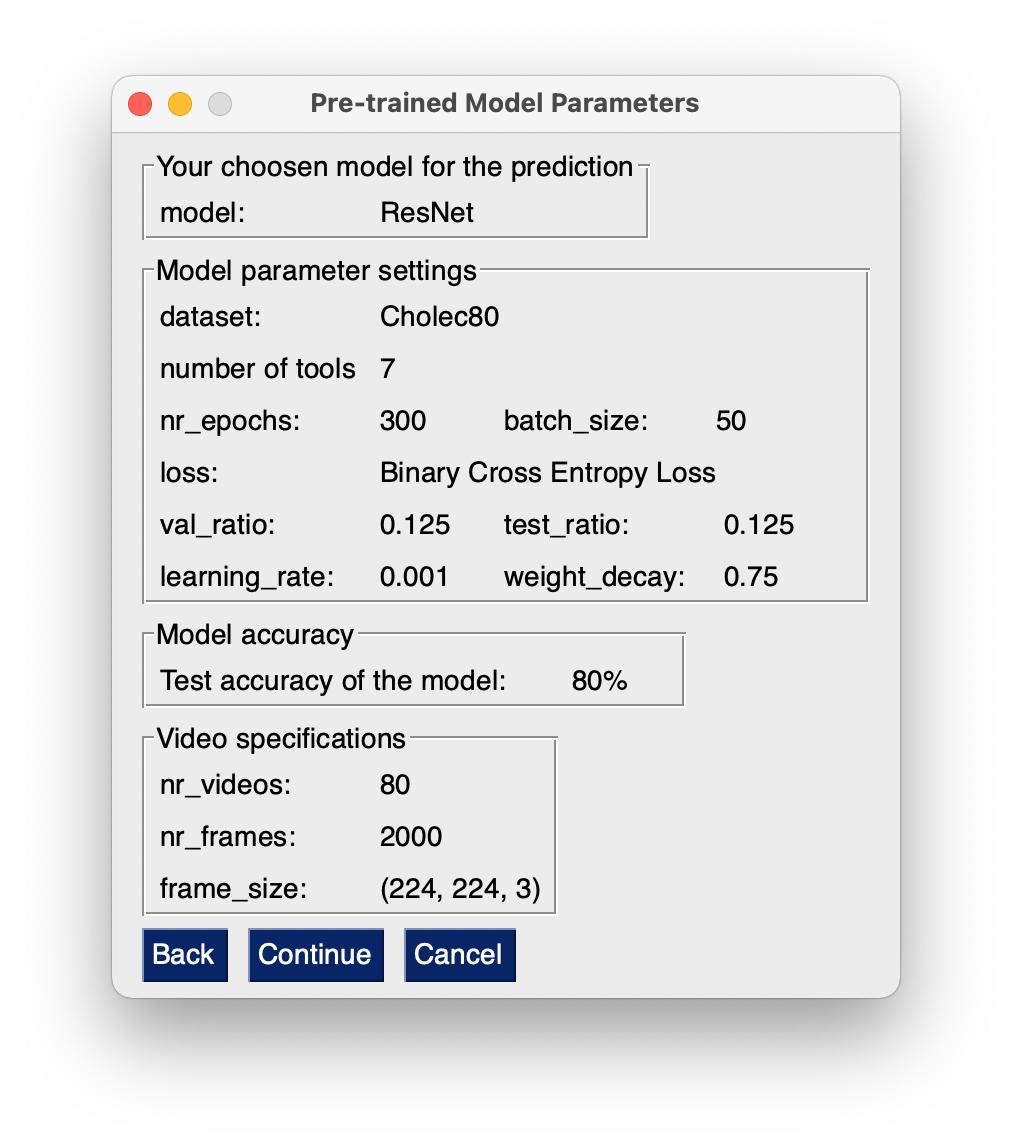
\includegraphics[width = 0.7\linewidth]{Parameter_window.jpg}
    \caption{Window that shows the parameters the selected model has been trained on with its test accuracy}
\end{figure}
\noindent

\subsubsection{Fourth Window - Results}
Once the user specified the model and device he/she wants to predict on, the prediction will start. In this case a progress bar will be shown to the user on which the progress can be seen:

\begin{figure}[H]
    \centering
    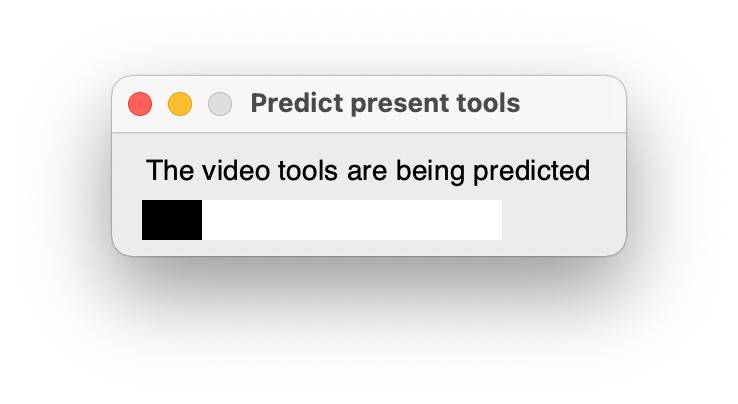
\includegraphics[width = 0.5\linewidth]{Loading_window.jpg}
    \caption{Progress bar indicating the progress of the prediction}
\end{figure}
\noindent
Once the computation is finished, the final window will appear, showing the results. In this window the predicted tools for each frame will be listed. The same output will be saved as a .json file after the user hits \texttt{Start again} to use a new video or \texttt{Finish} to exit the tool:

\begin{figure}[H]
    \centering
    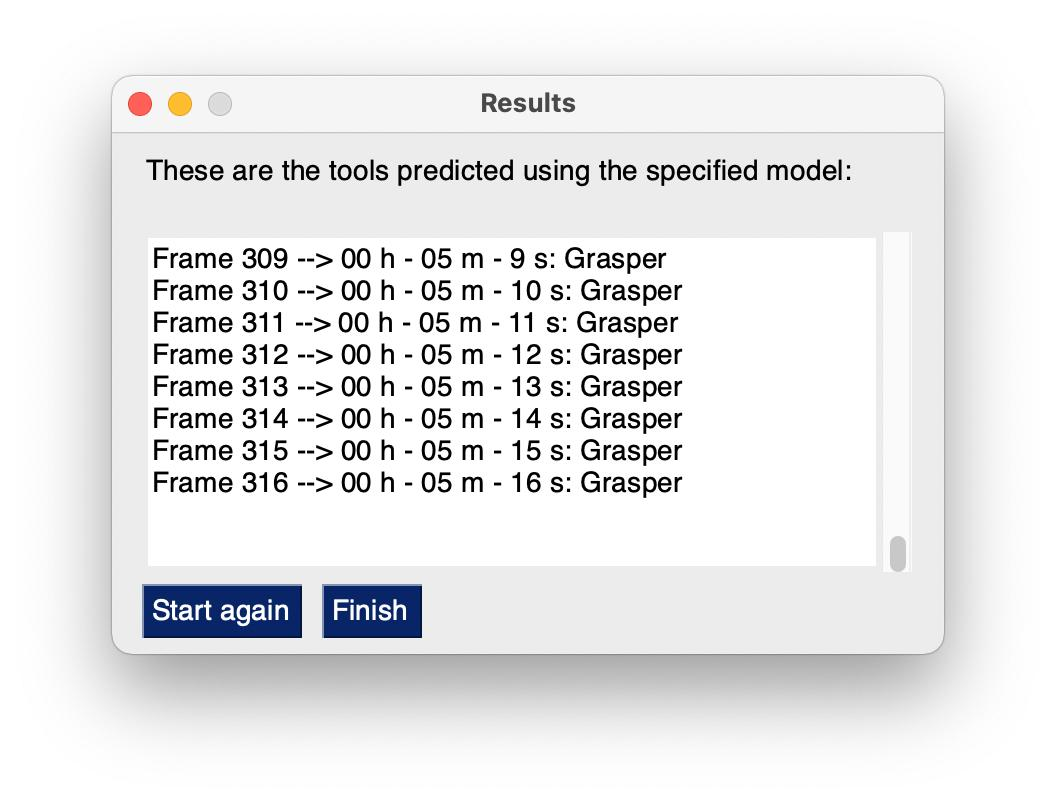
\includegraphics[width = 0.8\linewidth]{Results_window.jpg}
    \caption{Results window with output}
\end{figure}
\noindent

\end{document}